\chapter{Дослідження стійкості різницевих схем.  Метод фон Неймана.  Коефіцієнт та матриця переходу}

\shortLectureDescription{Метод фон Неймана. Коефіцієнт та матриця переходу. Явні та неявні різницеві схеми, алгоритми дослідження. Теореми про збіжність ряду Фур'є та стійкість явної та неявної різницевих схем}

\section{Метод фон Неймана дослідження стійкості срр із сталими коефіцієнтами}

\subsection{Подання функцій у вигляді рядів та інтегралів Фур'є}

Якщо вектор-функція $\vec u \left( \vec x \right)$ ($\vec x = (x_1, \ldots, x_d)$) з простору $B$ періодична за кожним з аргументів $x_j$ з періодом $L_j$, то її ряд Фур'є має вигляд
\begin{equation}
    \label{eq:4.1}
    \vec u \left( \vec x \right) = \frac{1}{\sqrt{L_1 \cdot \ldots \cdot L_d}} \sum_{\vec k \in L} \vec{\tilde{u}} \left( \vec k \right) e^{I \vec k \vec x},
\end{equation}
де $i = \sqrt{-1}$, $\vec k$ є $d$-вимірний вектор, який при підсумуванні пробігає множину $L$, складену з векторів $\vec k_j$, компоненти яких незалежно один від одного приймають всі можливі значення вигляду $\frac{2 \pi r_j}{L_j}$, де $r_j$ --- довільне ціле число.

\begin{definition}
	\emph{Векторний коефіцієнт Фур'є} $\vec{\tilde{u}} \left( \vec k \right)$, розглянутий як функція аргументу $\vec k$ на множині $L$, визначає точку в просторі $B'$:
    \begin{equation}
        \label{eq:4.2}
        \vec{\tilde{u}} \left( \vec k \right) = \frac{1}{\sqrt{L_1 \cdot \ldots \cdot L_d}} \int_0^L \vec u \left( \vec x \right) e^{-I \vec k \vec x} \diff \vec x.
    \end{equation}

    Тут позначено $\int_0^L \diff \vec x = \int_0^{L_1} \diff x_1 \ldots \int_0^{L_d} \diff x_d$.
\end{definition}

В просторах $B$ і $B'$ введемо середньоквадратичні норми за допомогою норми
\begin{equation*}
    \left\| \vec u \right\|^2 = \sum_{j = 1}^p |u_j|^2.
\end{equation*}

\begin{proposition}
    Тоді \emph{рівність Парсеваля}
    \begin{equation}
        \label{eq:4.3}
        \int_0^L \left\| \vec u \left( \vec x \right) \right\|^2 \diff \vec x = \sum_{k \in L} \left\| \vec{\tilde{u}} \left( \vec k \right) \right\|^2
    \end{equation}
    встановлює однозначну відповідність між елементами цих просторів із збереженням норми\footnote{Така відповідність носить назву ``ізоморфізм''.}. 
\end{proposition}

Довільну інтегровну з квадратом вектор-функцію $\vec u \left( \vec x \right)$ можна подати у вигляді інтегралу Фур'є
\begin{equation}
    \label{eq:4.4}
    \vec u \left( \vec x \right) = \frac{1}{\sqrt{(2 \pi)^d}} \int \vec{\tilde{u}} \left( \vec k \right) e^{I \vec k \vec x} \diff \vec k,
\end{equation}
де інтегрування ведеться по всьому простору змінних $k_1, \ldots, k_d$, а функція $\vec{\tilde{u}} \left( \vec k \right)$ визначається рівністю
\begin{equation}
    \label{eq:4.5}
    \vec{\tilde{u}} \left( \vec k \right) = \frac{1}{\sqrt{(2 \pi)^d}} \int \vec u \left( \vec x \right) e^{I \vec k \vec x} \diff \vec x.
\end{equation}

Рівність Парсеваля в цьому випадку має вигляд
\begin{equation}
    \label{eq:4.6}
    \int \left\| \vec u \left( \vec x \right) \right\|^2 \diff \vec x = \int \left\| \vec{\tilde{u}} \left( \vec k \right) \right\|^2 \diff \vec k.
\end{equation}

\begin{remark}
    Під функцією $e^A$, аргументом якої є $(p \times p)$-матриці, будемо розуміти степеневий ряд
    \begin{equation*}
        e^A = 1 + A + \frac{A^2}{2!} + \frac{A^3}{3!} + \ldots + \frac{A^n}{n!} + \ldots.
    \end{equation*}
\end{remark}

Для достатньо гладких функцій всі ці рівності можна розуміти буквально. Але якщо множини елементів просторів $B$ і $B'$ обмежити тільки такими функціями то може виявитись, що ці простори не будуть повними. Тому для збереження необхідного рівня строгості доцільно прийняти всі положення теорії гільбертового простору $L_2$. \medskip

Зокрема будемо:
\begin{itemize}
    \item вважати дві функції рівними, якщо вони різняться одна від одної на множині міри нуль;
    \item інтеграли розуміти як інтеграли Лебега;
    \item збіжність до границі --- як збіжність в середньо-квадратичному. 
\end{itemize}

Під рівністю \eqref{eq:4.1} будемо розуміти $\|u - u_n\| \to 0$ при $n \to \infty$, якщо під $u_n$ розуміємо послідовність частинних сум ряду, для яких індекс підсумування змінюється від $-n$ до $n$. Аналогічно, під рівністю \eqref{eq:4.4} розуміємо границю $\|u - u_K\| \to 0$ при $K \to \infty$, в якій $u_j$ --- це інтеграл, для якого кожна змінна $k_j$ пробігає інтервал $-K \le k_j \le K$. \medskip

При прийнятті цих умов простори $B$ і $B'$ є повними банаховими просторами. Перетворення \eqref{eq:4.2} відображає весь простір $B$ в $B'$ і в силу теореми Фур'є є оберненим по відношенню до \eqref{eq:4.1}, а за теоремою Рісса---Фішера, перетворення \eqref{eq:4.1} переводить весь простір $B'$ в $B$, так що довільна визначена на $L$ послідовність $\vec{\tilde{u}} \left( \vec k \right)$, для якої збігається сума в правій частині рівності \eqref{eq:4.3}, є послідовністю коефіцієнтів Фур'є деякої функції $\vec u \left( \vec x \right) \in B$. Аналогічно, \eqref{eq:4.4} в силу теореми Планшереля є взаємно однозначним відображенням простору $B'$ на простір $B$, а \eqref{eq:4.5} --- оберненим до нього. \medskip

Далі при використанні перетворення Фур'є ми будемо неявно використовувати усі прийняті положення, а під множиною $L$ розуміти або увесь простір змінних $k_1, \ldots, k_d$, або описану вище дискретну решітку.

\begin{definition}
    \emph{Носієм} функції називається замикання множини тих точок, у яких вона відмінна від нуля.
\end{definition}

\begin{definition}
    Кажуть, що функція \emph{має компактний носій}, якщо її носієм є компактна множина.
\end{definition}

\begin{remark}[щодо коректності постановок задач]
    Перша вимога коректності крайових задач про щільність області визначення розв'язуючого оператора $E_0(t)$ в $B$, випливає з того, що початковий елемент $\vec u \left( \vec x, 0 \right)$ можна як завгодно точно наблизити тригонометричним поліномом або функцію $\vec u \left( \vec x, 0 \right)$ можна подати за допомогою перетворення Фур'є з компактним носієм. Такі початкові множини у обох випадках є щільними в $B$. \medskip

	Друга умова коректності у даному разі полягає в тому, що $\left\| e^{t p(I k)} \right\|$ повинна бути рівномірно обмеженою за усіма $k$, тоді
	\begin{equation*}
	    \|E(t)\| = \max_{k \in L} \left\| e^{t p(I k)} \right\|.
	\end{equation*}

    Виконання цієї умови потрібно перевіряти у кожному конкретному випадку окремо.
\end{remark}

Надалі ми будемо вважати, що маємо справу тільки з коректно поставленими задачами. У цьому випадку вибір банахового простору є частиною постановки задачі. Як ми уже бачили вище, вибір середньоквадратичної метрики визначається бажанням використати перетворення Фур'є, але для самого розв'язку $\vec u$, норма якого визначена як середньоквадратична, залишається ще значна свобода вибору. Це відноситься до випадків, коли перед застосуванням загальної теорії диференціальних рівнянь, рівняння високого порядку приводиться до системи рівнянь першого порядку. Так у [5] розглянуто задачу про хвильовий рух, яка є коректною при одному простому виборі банахового простору і не коректною при іншому також простому його виборі. \medskip

Для цих простіших випадків перевірка коректності, як правило, порівняно не складна. Проте існують задачі, наприклад задача про багатовимірний рух рідких середовищ, для яких до нашого часу незрозуміло як коректно поставити крайову задачу, не використовуючи додаткових фізичних принципів.

Крім того ми будемо вважати, що усі неявні різницеві рівняння 
\begin{equation*}
    B_1 \vec u^{\,n + 1} - B_0 \vec u^{\,n} = 0,
\end{equation*}
тобто рівняння у яких оператор $B_1$ не є діагональною матрицею, мають єдиний розв'язок принаймні для умов періодичності за просторовими змінними.

\subsection{Умови стійкості чисельних алгоритмів}

Нехай тепер $\vec u^{\,n} = \vec u^{\,n}(\vec x)$ є наближенням розв'язку $\vec u(\vec x, n \Delta t)$ системи різницевих рівнянь 
\begin{equation*}
    B_1 \vec u^{\,n + 1} - B_0 \vec u^{\,n} = 0.
\end{equation*}

Ці різницеві рівняння можна записати у вигляді 
\begin{equation}
    \label{eq:4.7}
    \sum_{\beta \in N_1} B_1^\beta T^\beta \vec u^{\,n + 1} = \sum_{\beta \in N_0} B_0^\beta T^\beta \vec u^{\,n},
\end{equation}
де підсумування проведене за всіма точками шаблонів $N_1$ і $N_0$; через $T^\beta$ позначено складову різницевого оператора, яка замінює значення функції в точці $\vec x = (x_1, \ldots, x_d)$ на значення функції в деякій точці шаблона $N_j$ оператора $B_j$ ($j = 0, 1$):
\begin{equation*}
    (x_1 + \beta_1 \Delta x_1, \ldots, x_d + \beta_d \Delta x_d),
\end{equation*}
а компоненти векторного індексу $\beta = (\beta_1, \ldots, \beta_d)$ приймають певні цілі значення. Коефіцієнти матриці $B_1^\beta$ і $B_0^\beta$, які ставляться у відповідність значенням функції в кожній точці шаблона, можуть залежати від приростів координат $\Delta t$ і $\Delta x$, але не залежать від самих координат.

\begin{proposition}
    При виконанні таких умов щодо функцій $\vec u^{\,n}$ і $\vec u^{\,n + 1}$ можна застосувати перетворення Фур'є.
\end{proposition}

Нехай задача \eqref{eq:4.7} має розв'язок, тобто існує обмежений обернений оператор $B_1^{-1}$ і
\begin{equation}
    \label{eq:4.8}
    \vec u^{n + 1} = B \vec u^n, 
\end{equation}
де $B = B_1^{-1} C_0 = \sum_{\beta \in N} B^\beta T^\beta$, $N$ --- шаблон оператора $B$. 

\begin{remark}
    Уважаємо, що розв'язок задачі --- періодична вектор-функція. В іншому разі її можна продовжити в деяку область, таким чином, щоб в цій області вона стала періодичною.
\end{remark}

\begin{proposition}
    Відзначимо, що функцію $f$, визначену на напіввідкритому інтервалі довжини $2 \ell$, тобто на $[a, a + 2 \ell)$ або $(a, a + 2 \ell]$, можна продовжити (причому єдиним чином) на всю числову вісь так, що одержана функція буде періодичною з періодом $2 \ell$, а будь-яка періодична функція, яка має на проміжку  $(a, a + 2 \ell)$ не більше ніж скінчене число точок розривів і абсолютно інтегровна на цьому сегменті, у всіх внутрішніх точках диференційованості з цього сегмента може бути розвинутою в ряд Фур'є.
\end{proposition}

Уведемо банаховий простір $B'$ сіткових векторних функцій 
\begin{equation*}
    \vec \phi (m_s) = \begin{pmatrix} \xi^{(1)}(m_s) & \cdots & \xi^{(d)}(m_s) \end{pmatrix}^\intercal
\end{equation*} 
амплітудних членів $m_s$-тих гармонік розвинення розв'язку в збіжні ряди Фур'є 
\begin{equation}
    \label{eq:4.9}
    \vec u_i^{\,n + 1} = \sum_{s = 1}^d \sum_{m_s = -\infty}^\infty A(m_s) \vec \phi^{\,n + 1}(m_s) \exp \left\{ I \sum_{\ell = 1}^d i_\ell m_\ell h_\ell \right\},
\end{equation}
де $A(m_s)$ --- діагональна матриця, складена з коефіцієнтів розвинення вектор-функції $\vec u(x, 0)$ в ряди Фур'є, а $\vec \phi(m_s)$ --- вектори, які підлягають визначенню у процесі розв'язування різницевого рівняння \eqref{eq:4.8}:
\begin{multline*}
    \sum_{s = 1}^d \sum_{m_s = -\infty}^\infty A(m_s) \vec \phi^{\,n + 1}(m_s) \exp \left\{ I \sum_{\ell = 1}^d i_\ell m_\ell h_\ell \right\} = \\ 
    = B \left( \sum_{s = 1}^d \sum_{m_s = -\infty}^\infty A(m_s) \vec \phi^{\,n}(m_s) \exp \left\{ I \sum_{\ell = 1}^d i_\ell m_\ell h_\ell \right\} \right).
\end{multline*}

Оскільки оператор $B$ лінійний і $B^\beta$ не залежить від координат, то обидві частини рівняння мають типовий множник 
\begin{equation*}
    \exp\left\{I \sum_{\ell = 1}^d i_\ell m_\ell h_\ell \right\} \ne 0.
\end{equation*}

Розділивши обидві частини останнього рівняння на цей множник, одержимо
\begin{equation*}
    H_1 \vec \phi^{\,n + 1} \left( \vec k \right) - H_0 \vec \phi^{\,n} \left( \vec k \right) = 0,    
\end{equation*}
де
\begin{equation*}
    H_1 = \sum_{\beta \in N_1} B_1^\beta \exp\{ I (k_1 \beta_1 \Delta x_1 + \ldots + k_d \beta_d \Delta x_d) \}
\end{equation*}
і
\begin{equation*}
    H_0 = \sum_{\beta \in N_0} B_0^\beta \exp\{ I (k_1 \beta_1 \Delta x_1 + \ldots + k_d \beta_d \Delta x_d) \}.
\end{equation*}
	 
Тоді оператори $H_1$ і $H_0$ не залежать від $x_s$ та $t$ і залежать тільки від $\Delta t$ та $m$ для всіх $s$. Якщо матриця $H_1$ має обернену і виконується умова узгодженості розв'язку різницевого рівняння \eqref{eq:4.8} з початковою умовою, тобто $\| \vec \phi^0 \| = 1$, то з останнього рівняння маємо рекурентну формулу для визначення $\vec \phi(m_s)$:
\begin{equation}
    \label{eq:4.10}
    \vec \phi^{\,n + 1} (m_s) = G(m_s, \Delta t, \Delta x) \vec \phi^{\,n}(m_s),
\end{equation}

\begin{definition}
    Тут $G(m_s, \Delta t, \Delta x) = H_1^{-1} H_0$ --- \emph{матриця переходу}.
\end{definition}

Оскільки рівність \eqref{eq:4.10} є аналогом рівності $u^{n + 1} = C(\Delta t) u^n$ в просторі $B$ і визначає в просторі перетворень Фур'є $B'$ оператор, що відповідає оператору $C(\Delta t)$ в просторі $B$, то умова стійкості рівняння \eqref{eq:4.7} полягає в тому, що для деякого числа $\tau > 0$ нескінченна множина матриць $G^n(m_s, \Delta t, \Delta x)$ при $0 < \Delta t < \tau$, $0 \le n \Delta t \le T$ і $\forall \vec k \in L$ повинна бути рівномірно обмеженою. \medskip

Враховуючи збіжність ряду \eqref{eq:4.9}, після очевидних перетворень маємо
\begin{equation*}
    \sum_{s = 1}^d \sum_{m_s = -\infty}^\infty A(m_s) \exp \left\{ I \sum_{\ell = 1}^d i_\ell m_\ell h_\ell \right\} \left( \vec \phi^{\,n + 1} (m_s) - G(m_s, \Delta t, \Delta x) \vec \phi^{\,n} \right) = 0.
\end{equation*} 

\begin{theorem}
    Якщо норма матриці переходу менша від одиниці, а функції початкового розподілу розв'язку $\vec u(x, 0)$ розвиваються в абсолютно збіжний ряд Фур'є, то точний періодичний розв'язок різницевого рівняння \eqref{eq:4.8} із сталими коефіцієнтами може бути поданий у вигляді ряду Фур'є \eqref{eq:4.9}.
\end{theorem}

\begin{proof}
	Для доведення цього твердження обидві частини \eqref{eq:4.10} помножимо на
	\begin{equation*}
	    A(m_s) \exp\left\{ I \sum_{\ell = 1}^d i_\ell m_\ell h_\ell \right\},
	\end{equation*}
	і підсумуємо результат за всіма значеннями $m_s$ та $s$. Тоді, маємо
	\begin{multline*}
	    \vec u^{\,n + 1} = \sum_{s = 1}^d \sum_{m_s = -\infty}^\infty A(m_s) \vec \phi^{\,n + 1}(m_s) \exp \left\{ I \sum_{\ell = 1}^d i_\ell m_\ell h_\ell \right\} = \\ = \sum_{s = 1}^d \sum_{m_s = -\infty}^\infty A(m_s) G(m_s, \Delta t, \Delta x) \vec \phi^{\,n}(m_s) \exp \left\{ I \sum_{\ell = 1}^d i_\ell m_\ell h_\ell \right\}.
	\end{multline*}

    Отже
    \begin{equation*}
        \|\vec u^{n + 1}\| \le \sum_{s = 1}^d \sum_{m_s = -\infty}^\infty \|A(m_s)\| \cdot \|G(m_s, \Delta t, \Delta x)\| \cdot \|\vec \phi^{\,n}(m_s)\| \le q^n \sum_{s = 1}^d \sum_{m_s = -\infty}^\infty \|A(m_s)\|.
    \end{equation*}

	Оскільки $q = \max_{m_s} \|G(m_s, \Delta t, \Delta x)\| \le 1$, а ряд Фур'є для початкової функції абсолютно збіжний, то остання нерівність є мажорантою для збіжності ряду \eqref{eq:4.9}.  \medskip

	Отже ряд \eqref{eq:4.9} збіжний, задовольняє початкові умови різницевої задачі та різницеве рівняння \eqref{eq:4.8} оскільки вектори $\vec \phi(m_s)$ є розв'язками різницевого рівняння \eqref{eq:4.10}. Тобто він є точним розв'язком задачі \eqref{eq:4.7}, а умова 
	\begin{equation*}
	    q = \max_{m_s} \|G(m_s, \Delta t, \Delta x)\| \le 1
	\end{equation*}
    є необхідною умовою стійкості різницевої схеми \eqref{eq:4.7}.
\end{proof}

Тут і далі норму лінійного оператора $P$, заданого в $B'$ за допомогою матриці $A \left( \vec k \right)$ визначаємо так 
\begin{equation*}
    \|P\| = \max_{\vec k \in L} \left\| A\left(\vec k\right)\right\|,
\end{equation*}
де при фіксованому $\vec k$
\begin{equation*}
    \left\|A\left(\vec k\right)\right\| = \max_{|\vec V| = 1} \left| \left( A\left( \vec k \right), \vec V \right) \right| = \max_{\vec V \ne 0} \frac{\left| \left( A\left( \vec k\right), \vec V\right)\right|}{\left| \vec V \right|},
\end{equation*}
а під $|\cdot|$ розуміємо норму в евклідовому векторному просторі.

\begin{proposition}
    Виконання нерівності 
    \begin{equation*}
        \rho (G^n(m_s, \Delta t, \Delta x)^n ) = \max_j |\lambda_j| \le 1 + O(\Delta t)
    \end{equation*}
    при $0 < \Delta t < \tau$, $0 \le n \Delta t \le T$  і $\forall \vec k \in L$, де $\lambda_j$ --- власні числа матриці $G(m_s, \Delta_t, \Delta x)$, є \emph{необхідною умовою стійкості фон Неймана}. 
\end{proposition}

Таке визначення стійкості при малих $\tau$ допускає скінчене зростання значення похибки за часом. \medskip

Якщо матриця $G(m_s, \Delta t, \Delta x)$ нормальна, то умова фон Неймана є не тільки необхідною, але й достатньою умовою. \medskip

Зокрема, при $p = 1$, тобто коли матриця переходу вироджується у множник переходу, умова фон Неймана для двошарової різницевої схеми з однією залежною змінною є необхідною і достатною умовою стійкості. \medskip

Оскільки 
\begin{equation*}
     \rho (G(m_s, \Delta t, \Delta x) ) \le  \| G(m_s, \Delta t, \Delta x) \|_{B'},
\end{equation*}
то розв'язок відповідного різницевого рівняння стійкий, якщо для деякого додатного числа $M$ і деякого $\tau > 0$ при $0 < \Delta t < \tau$ виконується нерівність
\begin{equation}
    \label{eq:4.11}
    \| G(m_s, \Delta t, \Delta x) \|_{B'} \le 1 + M \Delta t.
\end{equation}

В цьому випадку при $0 \le n \Delta t \le T$, $0 < \Delta t < \tau$ маємо  
\begin{equation*}
    \| G(m_s, \Delta t, \Delta x) \|_{B'} \le e^{M T}.
\end{equation*}

Малі збурення оператора $C(\Delta t)$ не порушують стійкості розв'язку різницевого оператора, що випливає з твердження.

\begin{theorem}[Крайса]
    Якщо розв'язок різницевого рівняння $\vec u^{\,n + 1} = C(\Delta t) \vec u^{\,n}$ стійкий, а сімейство операторів $Q(\Delta t)$ --- обмежене, то розв'язки рівнянь 
	\begin{equation*}
	    \vec u^{\,n+1} = ( C(\Delta t) + \Delta t Q(t) \Delta) \vec u^{\,n}
	\end{equation*}
    також стійкі.
\end{theorem}

У ряді випадків уводиться більш жорсткої умови, а саме $\max_j |\lambda_j| \le 1$. Це виправдовується тим, що у цих випадках граничні умови задачі не залежать від часу, тобто розв'язок задачі прямує до деякої стаціонарної функції не зростаючи. 

\begin{definition}
    Кажуть, що розв'язок різницевої задачі \emph{слабко стійкий}, якщо роз\-в'я\-зу\-ю\-чий оператор схеми задовольняє нерівності
    \begin{equation*}
        \|C^n(\Delta t)\| \le \const (\Delta t)^{-\alpha} = \const n^\alpha,
    \end{equation*}
    при $0 \le n \Delta t \le T$ та $0 < \Delta t < \tau$ для деякого фіксованого скінченого $\alpha \ge 0$ (традиційно $\alpha = 0$).
\end{definition}

Деякі визначення стійкості дозволяють розв'язку задачі бути більш чутливий до збурень. Так, якщо замість рівномірної обмеженості операторів $C^n(\Delta t)$ вимагається щоб їх зростання за нормою не перевищувало швидкість зростання деякого степеня $1/\Delta t$ при $\Delta t \to 0$, то просте збурення може привести до невиправданого зростання норм відповідної множини операторів переходу. \medskip

Якщо для крайової задачі область визначення оператора $E_0(t)$ щільна в $B$, але $E_0(t)$ не обмежений ні в одному з інтервалів $0 < t < \tau$, то не існує різницевої схеми, апроксимація якої була б узгодженою з цією задачею і стійкою. \medskip

При дослідженні стійкості розв'язків практичних задач необхідно слідкувати, щоб обмеження, які накладаються на початкову функцію, виконувались для розв'язку цієї задачі. \medskip

Резюмуючи, доцільно відзначити, що існують випадки, коли жодне з наведених нами визначень стійкості різницевих схем не може бути використане для практичних задач. Такою задачею є, наприклад, задача про спільне розповсюдження звуку та теплоти та інші [5].

\section{Приклади застосування методу фон Неймана}

\begin{example}
    Розглянемо початково-крайову задачу теплопровідності
    \begin{equation*}
        \frac{\partial u}{\partial t} = \alpha \frac{\partial^2 u}{\partial x^2}, \quad -\pi \le x \le \pi, \quad 0, \le t \le T, \quad \alpha = \const > 0,
    \end{equation*}
    \begin{equation*}
        u(x, 0) = \phi_0(x), \quad -\pi \le x \le \pi
    \end{equation*}
    з періодичним за просторовою змінною розв'язком.
\end{example}

\begin{proposition}
    Явна різницева схема, яка апроксимує цю диференціальну задачу, має вигляд
    \begin{equation*}
        \frac{u_i^{n + 1} - u_i^n}{\tau} = \alpha \frac{u_{i - 1}^n - 2 u_i^n + u_{i + 1}^n}{h^2}, \quad i = \overline{-M+1..M-1}, \quad n = \overline{1..N},
    \end{equation*}
    \begin{equation*}
        u_0^n = u_M^n, \quad u_1^n = u_{M + 1}^n, \quad n = \overline{1..N},
    \end{equation*}
    \begin{equation*}
        u_i^0 = \phi_0(i h), \quad i = \overline{-M+1..M-1}.
    \end{equation*}
\end{proposition}

Будемо уважати, що початкова функція $\phi_0(j h)$ розвивається у абсолютно збіжний ряд Фур'є, а сам розв'язок різницевої задачі можна подати у вигляді ряду Фур'є
\begin{equation}
    \label{eq:4.12}
    u_j^n = \sum_{m = -\infty}^\infty A_m V^n(m) \exp\{Imjh\}.
\end{equation}

Тут $I$ --- уявна одиниця ($I^2 = -1$), $A_m$ --- коефіцієнти Фур'є початкової функції $\phi_0(jh)$, $V(m)$ --- амплітудні коефіцієнти, які підлягають подальшому визначенню. \medskip

Нехай ряд, яким подано розв'язок, збіжний. Підставимо шуканий розв'язок у різницеве рівняння і враховуючи, що $\forall m$: $A_m \exp\{Imjh\} \ne 0$, для визначення $V(m)$ одержимо рівняння
\begin{equation*}
    V(m) - 1 = \frac{\alpha \tau}{h^2} \left( e^{Imh} - 2 + e^{-Imh} \right).    
\end{equation*}

Оскільки $e^{Imh} + e^{-Imh} = 2 \cos(mh)$, то
\begin{equation*}
    V = V(m) = 1 + d (\cos(m h) - 1), \quad d = \frac{2 \alpha \tau}{h^2}.
\end{equation*}

При виконанні останньої рівності сіткова функція \eqref{eq:4.12} буде розв'язком різницевого рівняння, задовольняти граничні умови періодичності, а також початкові умови. \medskip

Очевидно, що при $\max_m |V(m)| \le 1$ ряд Фур'є \eqref{eq:4.12} є збіжним. Легко також переконатися, що 
\begin{equation*}
    G = V(m) = 1 + d (\cos (m h) - 1)
\end{equation*}
є коефіцієнтом переходу розв'язку різницевого рівняння з часового шару $t_n = n \tau$ на шар $t_{n + 1} = (n + 1) \tau$, а умова $q = \max_m |G(m)| \le 1$  є умовою стійкості різницевого розв'язку. \medskip

Дійсно, обидві частини очевидної рівності
\begin{equation*}
    V^{n + 1}(m) = G V^n(m)
\end{equation*}
розділимо на $A_m \exp\{Imjh\} \ne 0$, підсумуємо результат за усіма $m$:
\begin{equation*}
    u_j^{n+1} = \sum_{m = -\infty}^\infty A_m V^{n+1}(m) \exp\{Imjh\} = \sum_{m=-\infty}^\infty A_mG(m)V^n(m)\exp\{Imjh\}
\end{equation*}
і зробимо оцінку
\begin{multline*}
    |u_j^{n+1}| = \left|\sum_{m = -\infty}^\infty A_m V^{n+1}(m) \exp\{Imjh\}\right| = \left|\sum_{m=-\infty}^\infty A_mG(m)V^n(m)\exp\{Imjh\}\right| \le \\ \le \max_m |G(m)|\cdot\left|\sum_{m=-\infty}^\infty A_mV^n(m)\exp\{Imjh\}\right|\leq|u_j^n|,
\end{multline*}
або
\begin{equation*}
    \|u^{n+1}\|=h\sqrt{\sum_{j=-M+1}^{M-1}(u_j^{n+1})^2} \le q^n h\sqrt{\sum_{j=-M+1}^{M-1}(u_j^0)^2} = q^n\|u^0\|.
\end{equation*}

Отже, $\|u^{n+1}\}\le q^n\|u^0\|$ і умовою стійкості різницевої схеми є $\max_m|G(m)| \le 1$. Звідси випливає, що для усіх $m$
\begin{equation*}
    -1 \le 1 + d (\cos(mh) - 1) \le 1
\end{equation*}
або  
\begin{equation*}
    -1 \le 1 - 2 d \sin^2(mh/2) \le 1
\end{equation*}
тобто $d \le 1/2$, або
\begin{equation*}
    \tau \le \frac{h^2}{2\alpha}.
\end{equation*}

\begin{example}
    До апроксимації початково-крайової задачі теплопровідності
    \begin{equation*}
        \frac{\partial u}{\partial t} = \alpha \frac{\partial^2 u}{\partial x^2}, \quad -\pi \le x \le \pi, \quad 0, \le t \le T, \quad \alpha = \const > 0,
    \end{equation*}
    \begin{equation*}
        u(x, 0) = \phi_0(x), \quad -\pi \le x \le \pi
    \end{equation*}
    з періодичним за просторовою змінною розв'язком застосуємо неявну різницеву схему
    \begin{equation*}
        \frac{u_i^{n + 1} - u_i^n}{\tau} = \alpha \frac{u_{i - 1}^{n + 1} - 2 u_i^{n + 1} + u_{i + 1}^{n + 1}}{h^2}, \quad i = \overline{-M+1..M-1}, \quad n = \overline{1..N},
    \end{equation*}
    \begin{equation*}
        u_0^n = u_M^n, \quad u_1^n = u_{M + 1}^n, \quad n = \overline{1..N},
    \end{equation*}
    \begin{equation*}
        u_i^0 = \phi_0(i h), \quad i = \overline{-M+1..M-1}.
    \end{equation*}
\end{example}

Як і раніше вважаємо, що початкова функція $\phi_0(jh)$ розвивається у абсолютно збіжний ряд Фур'є, а сам розв'язок різницевої задачі можна подати у вигляді ряду Фур'є
\begin{equation}
    \label{eq:4.13}
    u_j^n = \sum_{m = -\infty}^\infty A_m V^n(m) \exp\{Imjh\}.
\end{equation}

Після підстановки шуканого розв'язку у різницеве рівняння і врахування рівнос, що $A_m \exp\{Imjh\} \ne 0$, для визначення $V(m)$ маємо рівність
\begin{equation*}
    V(m) = (1 + d(1 - \cos(mh)))^{-1}.
\end{equation*}

Очевидно, що у цьому випадку $\max_m |V(m)| \le 1$ і отже ряд Фур'є \eqref{eq:4.13} є збіжним, а функція \eqref{eq:4.13} розв'язком різницевої задачі. \medskip

Оскільки модуль коефіцієнта переходу $|G| = |V(m)|$ розв'язку різницевого рівняння з часового шару $t_n = n \tau$ на шар $t_{n+1} = (n + 1) \tau$ менший від одиниці для усіх $m$, то різницева схема буде безумовно стійкою. 

\begin{example}
    Розглянемо задачу Коші для рівняння конвективного переносу
	\begin{equation*}
	    \frac{\partial u}{\partial t} = -k \frac{\partial u}{\partial x}, \quad u(x, 0) = u_0, \quad - \infty < x < \infty, \quad 0 < t < \infty. 
	\end{equation*} 
\end{example}

Запишемо для неї явну центрально різницеву схему 
\begin{equation*}
    \frac{u_i^{n + 1} - u_i^n}{\tau} = -k \frac{u_{i + 1}^n - u_{i - 1}^n}{2 h}.
\end{equation*}

Стійкість цієї схеми дослідимо застосовуючи метод фон Неймана. Розв'язок задачі будемо шукати у вигляді ряду Фур'є \eqref{eq:4.13}. Після підстановки розв'язку у різницеве рівняння і проведення перетворень аналогічних до проведених у першому прикладі, для визначення множника переходу одержимо 
\begin{equation*}
    V(m) = 1 - \frac{k \tau}{2 h} (e^{mh} - e^{-mh}) = 1 + IC \sin mh.
\end{equation*}

Тут $C = \frac{k \tau}{h}$ --- число Куранта. Оскільки 
\begin{equation*}
    |V(m)|^2 = 1 + C^2 \sin^2 mh \ge 1
\end{equation*}
то цей чисельний алгоритм не буде стійким ні при яких значення $\tau$ та $h$.

\begin{proposition}
    Стійкою для цієї задачі є різницева схема з різницями проти потоку. 
\end{proposition}

Для одновимірного хвильового рівняння цю різницеву схему можна подати як схему з односторонніми різницями першого порядку апроксимації за просторовими змінними:
\begin{equation*}
    \frac{u_i^{n + 1} - u_i^n}{\tau} = \begin{cases}
        -k \frac{u_i^n - u_{i - 1}^n}{h}, & k > 0, \\
        -k \frac{u_{i + 1}^n - u_i^n}{h}, & k < 0.
    \end{cases}
\end{equation*}

\begin{proposition}
    Така схема має перший порядок апроксимації.
\end{proposition}

Використовуючи метод фон Неймана, легко переконатися, що умовою стійкості цієї схеми буде $|C| \le 1$, де $C = \frac{k \tau}{h}$ --- число Куранта.

\begin{example}
	Для рівняння конвективного переносу
	\begin{equation*}
	    \frac{\partial u}{\partial t} = -k \frac{\partial u}{\partial x}
	\end{equation*}
    запишемо тришарову різницеву схему
	\begin{equation*}
	    \frac{u_i^{n + 1} - u_i^{n - 1}}{2 \Delta t} = - k \frac{u_{i + 1}^n - u_{i - 1}^n}{5\Delta x}.
	\end{equation*}
\end{example}

\begin{proposition}
    За допомогою безпосередньої перевірки легко переконатися, ця схема має другий порядок апроксимації за обома змінними. 
\end{proposition}

Дослідження цієї схеми проведемо за методом фон Неймана. Для цього записане різницеве рівняння подаємо у вигляді
\begin{equation*}
    u_i^{n + 1} = u_i^n - C(u_{i + 1}^n - u_{i - 1}^n),
\end{equation*}
де $C = \frac{u \delta t}{\Delta x}$ --- число Куранта. Після підстановки в останню формулу гармоніку ряду Фур'є \eqref{eq:4.13} та виконання елементарних перетворень, приходимо до рівності
\begin{equation*}
    V^{n + 1} = a V^n + V^{n - 1}
\end{equation*}
де $a = -2IC \sin \theta$, а $\theta = m \Delta x$. \medskip

Для того, щоб одержати рівняння для визначення матриці переходу додатково розглянемо тотожність
\begin{equation*}
    V^n = 1 \cdot V^n + 0 \cdot V^{n - 1}.    
\end{equation*}

Об'єднавши ці дві рівності одержуємо векторне рівняння
\begin{equation*}
    \begin{bmatrix}
        V^{n + 1} \\ V^n
    \end{bmatrix} = 
    \begin{bmatrix}
        a & 1 \\ 1 & 0
    \end{bmatrix}
    \begin{bmatrix}
        V^n \\ V^{n - 1}
    \end{bmatrix}.
\end{equation*}

Тут матриця 
\begin{equation*}
    G(m) = 
    \begin{bmatrix}
        a(m) & 1 \\ 1 & 0
    \end{bmatrix}
\end{equation*}
є матрицею переходу. \medskip

Використаємо відоме
\begin{proposition}
    Для стійкості багатошарової різницевої схеми спектральний радіус матриці переходу $\rho(G) = \max_j |\lambda_j|$ (тут $\lambda_j$ --- $j$-те власне значення матриці $G$) не повинен перевищувати одиниці. 
\end{proposition}

Отже, для установлення умови стійкості необхідно дослідити, при яких усі умовах розв'язки характеристичного рівняння 
\begin{equation*}
    \begin{vmatrix}
        a - \lambda & 1 \\ 1 & 0 - \lambda
    \end{vmatrix} = 0,
\end{equation*}
або
\begin{equation*}
    \lambda^2 - a \lambda - 1 = 0
\end{equation*}
менші від одиниці. \medskip

Оскільки $\lambda_\pm = (a \pm \sqrt{a^2 + 4}) / 2$, а $a = -2IC \sin\theta$, то при $C^2 \sin^2 \theta > 1$ власні числа матриці  $G$
\begin{equation*}
    \lambda_\pm = I (-C \pm \sqrt{C^2 \sin^2 \theta - 1})
\end{equation*}
є чисто уявними числами, модуль яких більший від одиниці. Якщо $C^2 \sin^2 \theta \le 1$, (оскільки умова стійкості повинна виконуватись для всіх гармонік ($\forall m$), це еквівалентно умові $|C| \le 1$) то 
\begin{equation*}
    |\lambda_\pm|^2 = \lambda \bar \lambda = 1
\end{equation*}
і отже, різницева схема буде стійкою при $C = 1$. \medskip

Робити висновок, що така умова є задовільною тільки в крайньому разі невірно. Це граничне значення умови стійкості є навіть бажаним в випадку, коли розв'язок початкового диференціального рівняння не затухає. Дійсно, рівняння конвективного переносу описує простий зсув довільного початкового розподілу $u(x, 0)$ функції із швидкістю конвекції $k$ ($k \tau = h$). Тобто за проміжок часу $\tau$ розв'язок переноситься з точки $(x - k \tau, t)$ у точку $(x, t + \tau)$ і при цьому маємо $u(x, t + \tau) = u(x - k \tau, t)$. Якщо $C = 1$, то запропонована тришарова різницева схема дає точний розв'язок задачі. Вибираючи $\tau = \Delta t$, маємо $x - k \tau = x - C \Delta x$, а отже, точний розв'язок диференціального рівняння на сітковій множині запишеться відповідно:
\begin{itemize}
    \item $u_{i + 1}^n = u_i^{n - 1}$ в точці $(x_i + \Delta x, t_n)$;
    \item $u_i^{n + 1} = u_{i - 1}^n$ в точці $(x_i, t_n + \Delta t)$.
\end{itemize}

Об'єднавши ці рівності приходимо до рівняння
\begin{equation*}
    u_i^{n + 1} = u_i^{n - 1} - u_{i + 1}^n + u_{i - 1}^n,
\end{equation*}
яке відповідає розглянутій трикроковій різницевій схеми при $C = 1$. Тобто у даному разі розв'язок різницевої задачі співпадає з точним розв'язком диференціальної. \medskip

Відмітимо, що при $k \ne \const$ досягти виконання умови $C = 1$ практично неможливо. \medskip

Суттєвим недоліком тришарових схем є те, що для знаходження розв'язку потрібно задавати не один початковий розподіл в момент часу $t = 0$, як це робиться для диференціальної задачі, а задавати значення на двох часових кроках $t_0$ та $t_1$. Тобто різницева рівняння є по суті рівнянням другого порядку і вимагає початкових умов, еквівалентних умовам $u(x, 0) = \phi(x)$ та $\left. \frac{\partial u}{\partial t} \right|_{t = 0} = \phi(x)$, які приводять до перевизначеності диференціальної задачі. Для подолання цієї проблеми використовують наближені значення шуканого розв'язку, одержаного за допомогою деякого двошарового різницевого методу. При цьому для збереження другого порядку точності розв'язку в двошаровій схемі використовують значно менший крок $\tau' = \tau / k$ і за значення $u_i^1$ приймають значення одержане в момент часу $k \tau '$.

\section{Аналіз стійкості за Хьортом}

Третій метод аналізу стійкості був запропонований Хьортом [1968]. У цьому методі члени, що входять у кінцево-різницеві рівняння, розкладаються в ряди Тейлора для того, щоб одержати диференціальне рівняння в частинних похідних. Стійкість потім визначається з відомих властивостей стійкості диференціальних рівнянь. (Аналогічний підхід до вивчення кінцево-різницевих рівнянь за допомогою отриманих у такий спосіб диференціальних рівнянь був використаний у роботі Сайруса й Фалтона [1967] для дослідження не стійкості, а точності кінцево-різницевих методів, застосовуваних для еліптичних рівнянь.) \medskip

Розглянемо знову схему з різницями вперед за часом і центральними різницями по просторовій змінній для модельного рівняння, що включає конвективний і дифузійний члени, припускаючи, що $u$ постійно:
\begin{equation}
    \label{eq:3.114}
    \frac{\zeta_i^{n + 1} - \zeta_i^n}{\Delta t} = -u\left(\frac{\zeta_{i + 1}^n - \zeta_{i - 1}^n}{2\Delta x}\right) + \alpha \left( \frac{\zeta_{i + 1}^n - 2 \zeta_i^n + \zeta_{i - 1}^n}{\Delta x^2}\right).
\end{equation}

Розкладемо кожний член рівняння \eqref{eq:3.114} у ряди Тейлора в околі точки $(x, t)$, тобто відносно $\zeta_i^n$ тоді
\begin{align}
    \label{eq:3.115}
    \zeta_i^{n + 1} &= \zeta_i^n + \Delta t \left. \frac{\partial \zeta}{\partial t} \right|_i^n  + \half \Delta t^2 \left. \frac{\partial^2 \zeta}{\partial t^2} \right|_i^n + O(\Delta t^3), \\
    \label{eq:3.116}    
    \zeta_{i \pm 1}^n &= \zeta_i^n \pm \Delta x \left. \frac{\partial \zeta}{\partial x} \right|_i^n  + \half \Delta x^2 \left. \frac{\partial^2 \zeta}{\partial x^2} \right|_i^n \pm O(\Delta t^3).
\end{align}

Підставляючи ці розкладання в \eqref{eq:3.114} і приводячи подібні члени, одержуємо
\begin{multline}
    \label{eq:3.117}
    \frac{1}{\Delta t} \left( \Delta t \left. \frac{\partial \zeta}{\partial t} \right|_i^n + \half \Delta t^2 \left. \frac{\partial^2 \zeta}{\partial t^2} \right|_i^n + O(\Delta t^3) \right) = \\ = \frac{u}{2\Delta x} \left( 2 \Delta x \left. \frac{\partial \zeta}{\partial x} \right|_i^n + O(\Delta x^3) \right) + \frac{\alpha}{\Delta x^2} \left( \Delta x^2 \left. \frac{\partial^2 \zeta}{\partial x^2} \right|_i^n + O(\Delta x^4) \right)
\end{multline}
або, опускаючи індекси $i$ і $n$,
\begin{equation}
    \label{eq:3.118}
    \frac{\partial \zeta}{\partial t} + \frac{\Delta t}{2} \frac{\partial^2 \zeta}{\partial t^2} = - u \frac{\partial \zeta}{\partial x} + \alpha \frac{\partial^2 \zeta}{\partial x^2} + O(\Delta t^2, \Delta x^2).
\end{equation}

При $\Delta t \to 0$, $\Delta x \to 0$ це рівняння переходить у вихідне диференціальне рівняння в частинних похідних \eqref{eq:2.18}. Але при $\Delta t > 0$ рівняння \eqref{eq:3.118} приймає вид
\begin{equation}
    \label{eq:3.119}
    \frac{\Delta t}{2 \alpha} \frac{\partial^2 \zeta}{\partial t^2} - \frac{\partial^2 \zeta}{\partial x^2} + \frac{1}{\alpha} \frac{\partial \zeta}{\partial t} + \frac{u}{\alpha} \frac{\partial \zeta}{\partial x} = 0.
\end{equation}

Це рівняння, отримане збереженням усіх членів першого порядку в розкладаннях ряду Тейлора, є гіперболічним

\begin{figure}[H]
    \centering
    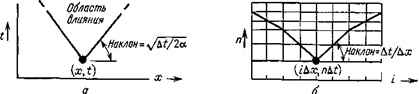
\includegraphics{{img/07/3.9}.png}
    \caption{Область впливу точки $(x, t)$ для рівняння \eqref{eq:3.118} гіперболічного типу, а --- область впливу для диференціального рівняння; б --- область впливу для скінчено-різницевого рівняння.}
    \label{fig:3.9}
\end{figure}

Як показано на мал.~\ref{fig:3.9}.а, для таких рівнянь існує область впливу довільної точки $(x, t)$, що обмежена характеристиками, що мають нахил $\pm\sqrt{\frac{\Delta t}{2\alpha}}$ і проходять через цю точку. Збурювання, що виникають у точці $(x,t)$, проявляються тільки усередині цієї області. 

\begin{definition}
    Частину площини $(x,t)$, розташовану поза цією областю, іноді називають \emph{зоною мовчання}.
\end{definition}

Для скінчено-різницевого рівняння \eqref{eq:3.114} також існує область впливу. Кожне нове розраховане значення $\zeta_i^{n + 1}$ залежить від значень $\zeta_{i\pm1}^n$ у сусідніх точках $i\pm1$ у попередній момент часу. Інакше кажучи, кожне значення $\zeta_i^n$ впливає на значення $\zeta_{i\pm1}^{n+1}$ в сусідніх точках на наступному шарі за часом. Цей вплив у свою чергу поширюється на значення $\zeta_{i\pm2}^{n+2}$ і т.д. Таким чином, область впливу дискретизованого рівняння \eqref{eq:3.118} обмежується скінчено-різницевими ``характеристичними лініями'' з нахилом  $\frac{\Delta t}{\Delta x}$ (див. мал..~\ref{fig:3.9}.б). Умова Куранта (Курант, Фрідріху й Леви [1928]) стійкості скінчено-різницевого аналога таких гіперболічних рівнянь вимагає, щоб область впливу скінчено-різницевого рівняння принаймні містила в собі область впливу диференціального рівняння. З мал.~\ref{fig:3.9} видно, що це накладає умову
\begin{equation*}
    \frac{\Delta t}{\Delta x} \le \sqrt{\frac{\Delta t}{2 \alpha}}
\end{equation*}
або
\begin{equation}
    \label{eq:3.120}
    \Delta t \le \half \frac{\Delta x^2}{\alpha}.
\end{equation}

Але це обмеження на $\Delta t$ в точності збігається з обмеженням, обумовленим дифузійним членом у рівнянні й отриманим раніше з аналізу стійкості як за допомогою методу дискретних збурювань, так і за допомогою методу фон Неймана. \medskip

Щоб визначити іншу необхідну умову стійкості, обчислимо член $\frac{\partial^2 \zeta}{\partial t^2}$ у рівнянні \eqref{eq:3.119}, диференціюючи вихідне диференціальне рівняння з урахуванням припущення $u = \const$:
\begin{align}
 	\label{eq:3.121}
 	\frac{\partial \zeta}{\partial t} &= -u\frac{\partial \zeta}{\partial x} + \alpha\frac{\partial^2 \zeta}{\partial x^2}, \\
 	\label{eq:3.122}
 	\frac{\partial^2 \zeta}{\partial t^2} &= -u\frac{\partial^2 \zeta}{\partial t \partial x} + \alpha\frac{\partial^3 \zeta}{\partial t \partial x^2}.
\end{align}

Змінюючи порядок диференціювання й підставляючи $\frac{\partial \zeta}{\partial t}$ з вихідного диференціального рівняння в частинних похідних,
отримаємо
\begin{align}
    \label{eq:3.123}
    \frac{\partial^2 \zeta}{\partial t^2} &= - u \frac{\partial}{\partial x} \left( -u\frac{\partial \zeta}{\partial x} + \alpha \frac{\partial^2}{\partial x^2} \right) + \alpha \frac{\partial^2}{\partial x^2} \left( - u \frac{\partial \zeta}{\partial x} + \alpha \frac{\partial^2 \zeta}{\partial x^2}\right), \\
 	\label{eq:3.124}
    \frac{\partial^2 \zeta}{\partial t^2} &= u^2 \frac{\partial^2}{\partial x^2} -2u\alpha \frac{\partial^3 \zeta}{\partial x^4} + \alpha^2 \frac{\partial^4 \zeta}{\partial x^4}.
\end{align}

Підставляючи цей вираз в \eqref{eq:3.119} і перетворюючи результат, одержуємо
\begin{equation}
    \label{eq:3.125}
    \frac{\partial \zeta}{\partial t} = -u \frac{\partial \zeta}{\partial z} + \left( \alpha - \frac{u^2 \Delta t}{2} \right) \frac{\partial^2 \zeta}{\partial x^2} + u \alpha \Delta t \frac{\partial^3 \zeta}{\partial x^3} - \frac{\alpha^2 \Delta t}{2} \frac{\partial^4 \zeta}{\partial x^4}.
\end{equation}

Ідучи за Хьортом [1968], відкидаємо в рівнянні \eqref{eq:3.125} вищі похідні й зберігаємо перші й другі похідні по кожній незалежній змінній ($x$ і $t$), що дає корисне диференціальне наближення. Воно має сенс із двох причин. По-перше, похідні вищих порядків звичайно менші. По-друге, a posteriori відомо, що умова стійкості, отримана в результаті цього аналізу, буде сильніше за обмеження, що накладається на крок за часом при наявності тільки дифузійного члена, лише для течій з малою в'язкістю, тобто для $\alpha \ll u$, коли коефіцієнти при вищих похідних у рівнянні \eqref{eq:3.125} стають малими. У результаті виходить диференціальне наближення
\begin{equation}
 	\label{eq:3.126}
 	\frac{\partial \zeta}{\partial t} = -u \frac{\partial \zeta}{\partial x} + \alpha_{\text{еф}} \frac{\partial^2 \zeta}{\partial x^2}.
\end{equation}
де
\begin{equation}
 	\label{eq:3.127}
 	\alpha_{\text{еф}} = \alpha - \frac{u^2 \Delta t}{2}.
\end{equation}

\begin{definition}
    Оскільки рівняння \eqref{eq:3.126} еквівалентно вихідному модельному диференціальному рівнянню, будемо називати $\alpha_{\text{еф}}$ \emph{ефективною в'язкістю}.
\end{definition}

З математичної (і фізичної) точки зору роль в'язкості (дифузії) полягає в ``розмазуванні'' (дифузії) збурювання величини $\zeta$, у прагненні зробити розподіл $\zeta$; однорідним. Негативна в'язкість фізично неможлива, тому що вона приводила б до концентрації будь-яких малих збурень, що виникли в однорідному розподілі, і створювала б у такий спосіб монотонну нестійкість. Для стійкості необхідно, щоб виконувалася умова $\alpha_{\text{еф}} \ge 0$, або умова $\Delta t \le \frac{2 \alpha}{u^2}$, що співпадає з умовою, %\eqref{eq:3.113}
отриманою за допомогою методу фон Неймана. У комбінації з умовою \eqref{eq:3.120} вона включає умову Куранта $C = \frac{u \Delta t}{\Delta x} \le 1$. Цей аналіз не знімає обмеження %\eqref{eq:3.112} 
на сіткове число Рейнольдса й тому забезпечує необхідні, але не достатні умови стійкості для модельного рівняння з конвективним і дифузійним членами.

\begin{exercise}
    Повторити попередні дві вправи по визначенню умові стійкості для схеми з різницями проти потоку, використовуючи метод Хьорта.
\end{exercise}

\section{Завдання для самостійної роботи}

\shortHomeworkDescription{Побудувати та дослідити стійкість різницевих схем, які апроксимують рівняння дифузійного та конвективного переносу з двома та трьома просторовими змінними. Визначити, які з них будуть консервативними та транспортивними.}
